\documentclass[]{beamer}
\usepackage{xmpmulti}
\usepackage{psfrag}
\usepackage{xcolor}
\newcommand{\owner}{\mathcal{O}}
\newcommand{\manager}{\mathcal{M}}

\mode<presentation>
{\usetheme{Boadilla}  % very plain
}

\usepackage{xcolor}

\usepackage{amssymb,amsmath,amsthm}
\usepackage{boxedminipage}

\usepackage{tikz}
\usepackage{tikzpeople}

\usetikzlibrary{snakes}
\usetikzlibrary{backgrounds} 
\usepgflibrary{shapes.geometric}
\usepgflibrary{shapes.misc}
\usetikzlibrary{shapes.callouts}
\usepackage{pgfmath}


%%\newcommand{\view}{{\mathsf{view}}}
%%\newcommand{\DS}{{\mathsf{DS}}}
%%\newcommand{\emm}{{\mathsf{eMM}}}
%%\newcommand{\mm}{{\mathsf{MM}}}
%%\newcommand{\aep}{{\mathsf{aep}}}
%%\newcommand{\gep}{{\mathsf{gep}}}
%%\newcommand{\Dist}{{\mathsf{Dist}}}
%%\newcommand{\Hard}{{\mathsf{Hard}}}
%%\newcommand{\key}{\mathtt{key}}
%%\newcommand{\GetMM}{\mathsf{Get}}
%%\newcommand{\AddMM}{\mathsf{Add}}
%%
%%\newcommand{\vals}{\vec{\mathtt{v}}}
%%\newcommand{\val}{{\mathtt{v}}}
%%\newcommand{\op}{{\mathtt{op}}}

\newcommand{\calE}{\mathcal{E}}
\newcommand{\calH}{\mathcal{H}}
\newcommand{\calI}{\mathcal{I}}
\newcommand{\calQ}{\mathcal{Q}}
\newcommand{\db}{\mathsf{Data}}
\newcommand{\mem}{\mathsf{Mem}}
\newcommand{\vals}{\mathsf{Vals}}

\newcommand{\kh}{K^{\mathsf{h}}}
\newcommand{\ke}{K^{\mathsf{e}}}

%%\newcommand{\calL}{\mathcal{L}}
%%\newcommand{\lQ}{\calL^G}
%%\newcommand{\lU}{\calL^A}

\newcommand{\LMax}{\ell_{\text{max}}}

\setbeamercolor{uppercol}{fg=teal,bg=lightgray}%
\setbeamercolor{lowercol}{fg=olive,bg=lightgray!50}%

\newcommand{\aaa}{\mathsf{a}}
\renewcommand{\ggg}{\mathsf{g}}

\title[]{The Curse of the Length\\ The Case of Encrypted Multi-Maps}

\author{Giuseppe Persiano}

\institute[UNISA]{%
Universit\`a di Salerno\\ \qquad \\
}

\date[August 2020]{August, 2020}

\begin{document}

\newcommand{\zu}{\{0,1\}}
\newcommand{\ignore}[1]{}

%\ignore
{
\begin{frame}
  \titlepage



{\color{magenta}
{\em Mitigating Leakage in Secure Cloud-Hosted Data Structures: Volume-Hiding for
Multi-Maps via Hashing}
}

{\color{brown}
by Sarvar Patel, GP, Kevin Yeo, and Moti Yung 

CCS '19
}
\end{frame}



\begin{frame}
\frametitle{Start from the beginning}
\begin{center}
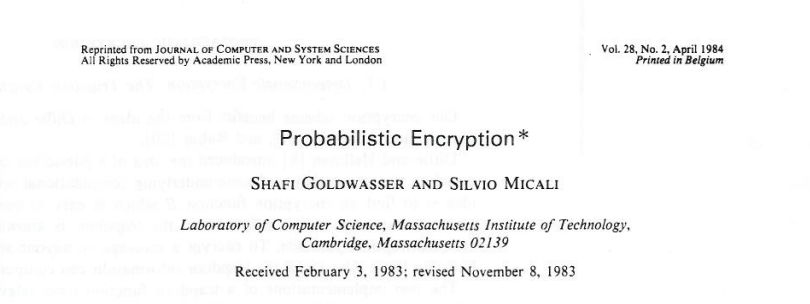
\includegraphics[width=4in]{imgs/GM1.png}
\end{center}
\end{frame}

\begin{frame}
\frametitle{Definition of Secure Encryption}
\begin{center}
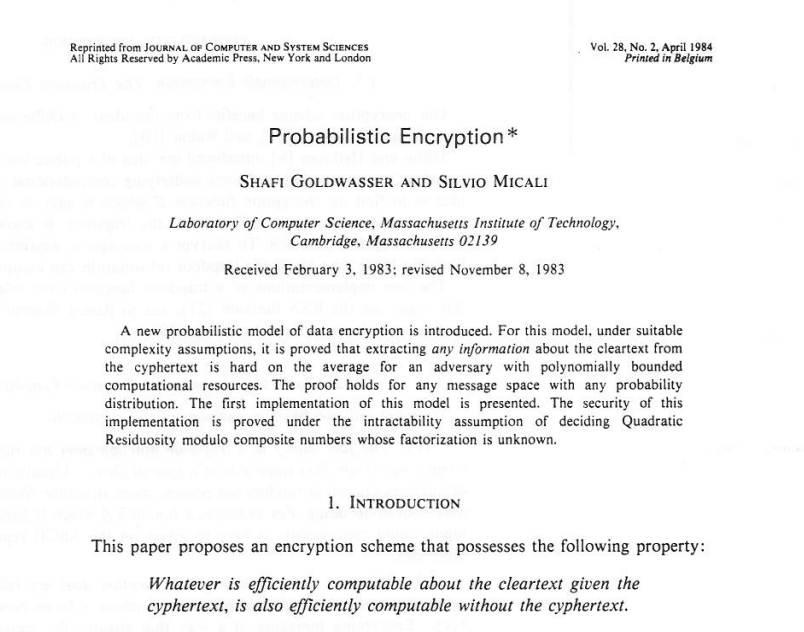
\includegraphics[width=4in]{imgs/GM2.png}
\end{center}
\end{frame}

\begin{frame}
\frametitle{The fine print}
\begin{center}
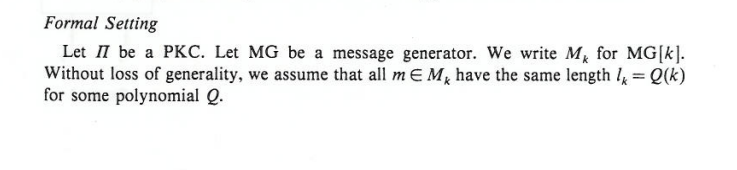
\includegraphics[width=4in]{imgs/GM3.png}
\end{center}

\only<2-3>{
Indeed WLOG:
}

\only<2>{
\vskip 1cm
{\color{white}{\em 
Just pad each message in the message space to the maximum length}}
}

\only<3>{
\vskip 1cm
{\color{magenta}{\em 
Just pad each message in the message space to the maximum length}}
}
\only<4>{
{\color{white}Indeed WLOG:}
\vskip 1cm
{\color{magenta}{\em 
Encryption necessarily leaks an upper bound on the length of the plaintext
}}
}
\end{frame}

\begin{frame}
\frametitle{Incompressibility}

\begin{block}{Fact of life}
{\color{magenta}{\bf
Encryption necessarily leaks an upper bound on the length of the plaintext
}}
\end{block}

\vfill
A direct consequence of Shannon/Kolmogoroff


\end{frame}
\begin{frame}
\frametitle{Structured Encryption
\hfill {\small Chase-Kamara 2010}}
\begin{itemize}[<+->]
\item Data is often organized in {\color{blue} Data Structures}
\vskip .3cm
\item For efficient retrieval 
\vskip .3cm
\item Storage is outsourced to untrusted server
    \begin{itemize}
        \item honest but {\color{blue} very} curious
    \end{itemize}
\end{itemize}
\end{frame}

%%\begin{frame}
%%\begin{tikzpicture}[font=\small]
%%\node[businessman,female,minimum size=1.5cm] (A) {};
%%\node[police,right=3cm of A,minimum size=1.5cm,mirrored] (B) {};
%%\node[anchor=north east] at (A.north west) (a2) {$(\mathsf{com},\mathsf{dec}) \gets \mathsf{Com}(a)$};
%%\node[anchor=south] at (a2.north) (a1) {$a\gets\{0,1\}$};
%%\node[anchor=south west] at (B.south east){$a \gets \mathsf{Opn}(\mathsf{com},\mathsf{dec})$};
%%\draw (A.35) edge[->] node[above] {$\mathsf{com}$} (B.145);
%%\node[anchor=south west] at (B.east |- B.180) {$b\gets\{0,1\}$};
%%\draw (A.0) edge[<-] node[above] {$b$} (B.180);
%%\draw (A.325) edge[->] node[above] {$\mathsf{dec}$} (B.215);
%%\draw (A.270) ++(0,-.5) node {$a\oplus b$} edge[<-] (A.270);
%%\draw (B.270) ++(0,-.5) node {$a\oplus b$} edge[<-] (B.270);
%%\end{tikzpicture}
%%\end{frame}

%AAAAA
\begin{frame}
\frametitle{(Plaintext) Multi-Maps}
\begin{tikzpicture}[
key/.style={rectangle,draw=green!50,fill=black!10,thick,minimum size=7mm,text=red},
simple/.style={rectangle,draw=yellow,fill=black!20,minimum size=7mm,text=magenta},
value/.style={rectangle,draw=black!50,fill=black!20,thick,minimum size=7mm,text=blue}]
\node at (1.0,1.0)  [key] (k1) {$L_1$}; 
\node [key, below=.2cm of k1] (k2) {$L_2$}; 
\node [below=.3cm of k2] (kdots) {$\ldots$}; 
\node [key, below=.8cm of k2] (kn) {$L_n$}; 
\node [above left=.05cm of k1]  (r1) {}; 
\node [below right=.05cm of kn] (r2) {}; 
\only<2>{
\draw (r1) [dashed,draw=teal]  rectangle (r2);
\node [simple, above right=1cm of r2] (lab) {$n$ {\em labels}};
\node [right=.1cm of k2]  (r3) {}; 
\draw [->,draw=brown,thick,out=190,in=10] (lab.west) to (r3);
}
\only<3>{
    \node [value,right=of k1] (val1) {$\vals(L_1)$};
    \draw [->,draw=brown,dashed] (k1.east) to (val1.west);
    \node [value,right=of k2] (val2) {$\vals(L_2)$};
    \draw [->,draw=brown,dashed] (k2.east) to (val2.west);
    \node [right=of kdots]  {$\ldots$};
    \node [value,right=of kn] (valn) {$\vals(L_n)$};
    \draw [->,draw=brown,dashed] (kn.east) to (valn.west);
    \node [simple, right=2cm of val2] (vals) {tuples of {\em values}};
    \draw [->,draw=brown,thick,out=170,in=10] (vals.west) to (val1);
    \draw [->,draw=brown,thick,out=180,in=0] (vals.west) to (val2);
    \draw [->,draw=brown,thick,out=190,in=10] (vals.west) to (valn);
}

\only<4->{
    \node [value,right=of k1]  (v11) {$V_{1,1}$};
    \node [value,right=.2cm of v11] (v12) {$V_{1,2}$};
    \node [value,right=.2cm of v12] (v13) {$V_{1,3}$};

    \node [value,right=of k2]  (v21) {$V_{2,1}$};

    \node [value,right=of kn]  (vn1) {$V_{n,1}$};
    \node [value,right=.2cm of vn1] (vn2) {$V_{n,2}$};
}
\only<5>{
    \node [below left=.01cm of v11]  (rl1) {}; 
    \node [above right=.05cm of v13]  (rl2) {}; 
    \draw (rl1) [dashed,draw=teal]  rectangle (rl2);
    \node [simple, below right=1cm of v13] (vals1) {$\vals(L_1)$};
    \node [below=.2cm of v12] (v12a) {};
    \draw [->,draw=brown,thick,out=170,in=260] (vals1.west) to (v12a);
}

\only<6>{
    \node [below left=.01cm of vn1]  (rln1) {}; 
    \node [above right=.05cm of vn2]  (rln2) {}; 
    \draw (rln1) [dashed,draw=teal]  rectangle (rln2);
    \node [simple, right=4cm of v21] (valsn) {$\vals(L_n)$};
    \node [above=.1cm of vn2] (vn2a) {};
    \draw [->,draw=brown,thick,out=260,in=80] (valsn.west) to (vn2a);
}
\only<7->{
\matrix[right=4cm of v11, draw=blue,dashed,font=\small]{
    \node[text=yellow,right] {\bf{Supported operations}};\\
    \node[text=red,right] {{Init}$((L_i,\vals(L_i))_i)$};\\
    \node[text=red,right] {{Get}$(L)\rightarrow\vals(L)$};\\
};
}
\only<8>
{
\matrix[right=4cm of vn1,draw=red,dashed]{
    \node [text=olive]  {\bf{Inverted index}};\\
    \node [text=olive]  {\quad Labels are keywords};\\
    \node [text=olive]  {\quad Values are documents};\\
};
}

\end{tikzpicture}

\end{frame}
%%\end{document}

\begin{frame}
\frametitle{Plaintext Multi-Maps}
\begin{tikzpicture}[
key/.style={rectangle,draw=green!50,fill=black!10,thick,minimum size=7mm,text=red},
value/.style={rectangle,draw=black!50,fill=black!20,thick,minimum size=7mm,text=blue}]

\node[alice,good,minimum size=1.5cm] (A) at (0,0){};
\node[below=of A] (AName) {\color{red}\huge User};
\node[bob,good,mirrored,minimum size=1.5cm,right=2.8cm of A] (B) {};
\node[right=3cm of AName] {\color{blue} \huge Cloud Manager};
\draw (5.5,-1.8) [dashed,draw=teal]  rectangle (10,1.7);
\node at (6.0,1.2)  [key] (k1) {$L_1$}; 
\node [value, right=.4cm of k1] (v11) {$V_{_{1,1}}$};
\node [value, right=.2cm of v11] (v12) {$V_{_{1,2}}$};
\node [value, right=.2cm of v12] (v13) {$V_{_{1,3}}$};
\draw [->,draw=brown,thick] (k1.east) to (v11.west);

\node [key, below=.2cm of k1] (k2) {$L_2$}; 
\node [value, right=.4cm of k2] (v21) {$V_{_{2,1}}$};
\draw [->,draw=brown,thick] (k2.east) to (v21.west);

\node [below=.3cm of k2] {$\ldots$}; 
\node [below=.3cm of v21] {$\ldots$}; 
\node [key, below=.8cm of k2] (kn) {$L_n$}; 
\node [value, right=.4cm of kn] (vn1) {$V_{_{n,1}}$};
\node [value, right=.2cm of vn1] (vn2) {$V_{_{n,2}}$};
\draw [->,draw=brown,thick] (kn.east) to (vn1.west);

\only<2>{\node[ellipse callout, fill=green!50, draw, callout absolute pointer={(A.north east)}] at (1.5,1.5) {$L_1$};}

\only<3->{
\draw [->,draw=brown,thick] (B.east) to [out=10,in=190] (k1.west);
}
\only<3>{
\node[ellipse callout, fill=green!50, draw, callout absolute pointer={(B.north west)}] at (1.5,1.5) {$V_{_{1,1}}$};}
\only<4->{\node [value,below=of AName] (v11d) {$V_{_{1,1}}$};}

\only<5>{\node[ellipse callout, fill=green!50, draw, callout absolute pointer={(B.north west)}] at (1.5,1.5) {$V_{_{1,2}}$};}
\only<6->{\node [value,right=.3cm of v11d] (v12d) {$V_{_{1,2}}$};}

\only<7>{\node[ellipse callout, fill=green!50, draw, callout absolute pointer={(B.north west)}] at (1.5,1.5) {$V_{_{1,3}}$};}
\only<8->{\node [value,right=.3cm of v12d] (v13d) {$V_{_{1,3}}$};}

\end{tikzpicture}
\end{frame}

\begin{frame}
\frametitle{Plaintext Multi-Maps with Evil Cloud Manager}
\begin{tikzpicture}[
key/.style={rectangle,draw=green!50,fill=black!10,thick,minimum size=7mm,text=red},
value/.style={rectangle,draw=black!50,fill=black!20,thick,minimum size=7mm,text=blue}]

\node[alice,good,minimum size=1.5cm] (A) at (0,0){};
\node[below=of A] (AName) {\color{red}\huge User};
\node[devil,mirrored,minimum size=1.5cm,right=2.8cm of A] (B) {};
\node[right=3cm of AName] {\color{blue} \huge Cloud Manager};
\draw (5.5,-1.8) [dashed,draw=teal]  rectangle (10,1.7);
\node at (6.0,1.2)  [key] (k1) {$L_1$}; 
\node [value, right=.4cm of k1] (v11) {$V_{_{1,1}}$};
\node [value, right=.2cm of v11] (v12) {$V_{_{1,2}}$};
\node [value, right=.2cm of v12] (v13) {$V_{_{1,3}}$};
\draw [->,draw=brown,thick] (k1.east) to (v11.west);

\node [key, below=.2cm of k1] (k2) {$L_2$}; 
\node [value, right=.4cm of k2] (v21) {$V_{_{2,1}}$};
\draw [->,draw=brown,thick] (k2.east) to (v21.west);

\node [below=.3cm of k2] {$\ldots$}; 
\node [below=.3cm of v21] {$\ldots$}; 
\node [key, below=.8cm of k2] (kn) {$L_n$}; 
\node [value, right=.4cm of kn] (vn1) {$V_{_{n,1}}$};
\node [value, right=.2cm of vn1] (vn2) {$V_{_{n,2}}$};
\draw [->,draw=brown,thick] (kn.east) to (vn1.west);

\only<2>{\node[ellipse callout, fill=green!50, draw, callout absolute pointer={(A.north east)}] at (1.5,1.5) {$L_1$};}

\only<3>{\node[ellipse callout, fill=green!50, draw, callout absolute pointer={(B.north west)}] at (1.5,1.5) {What???};}
\end{tikzpicture}
\end{frame}

\begin{frame}
\frametitle{Plaintext Multi-Maps with Honest-but-Curious Cloud Manager}

\begin{tikzpicture}[
key/.style={rectangle,draw=green!50,fill=black!10,thick,minimum size=7mm,text=red},
value/.style={rectangle,draw=black!50,fill=black!20,thick,minimum size=7mm,text=blue}]

\node[alice,good,minimum size=1.5cm] (A) at (0,0){};
\node[below=of A] (AName) {\color{red}\huge User};
\node[devil,good,mirrored,minimum size=1.5cm,right=2.8cm of A] (B) {};
\node[right=3cm of AName] {\color{blue} \huge Cloud Manager};
\draw (5.5,-1.8) [dashed,draw=teal]  rectangle (10,1.7);
\node at (6.0,1.2)  [key] (k1) {$L_1$}; 
\node [value, right=.4cm of k1] (v11) {$V_{_{1,1}}$};
\node [value, right=.2cm of v11] (v12) {$V_{_{1,2}}$};
\node [value, right=.2cm of v12] (v13) {$V_{_{1,3}}$};
\draw [->,draw=brown,thick] (k1.east) to (v11.west);

\node [key, below=.2cm of k1] (k2) {$L_2$}; 
\node [value, right=.4cm of k2] (v21) {$V_{_{2,1}}$};
\draw [->,draw=brown,thick] (k2.east) to (v21.west);

\node [below=.3cm of k2] {$\ldots$}; 
\node [below=.3cm of v21] {$\ldots$}; 
\node [key, below=.8cm of k2] (kn) {$L_n$}; 
\node [value, right=.4cm of kn] (vn1) {$V_{_{n,1}}$};
\node [value, right=.2cm of vn1] (vn2) {$V_{_{n,2}}$};
\draw [->,draw=brown,thick] (kn.east) to (vn1.west);

\only<2>{\node[ellipse callout, fill=green!50, draw, callout absolute pointer={(A.north east)}] at (1.5,1.5) {$L_1$};}

\only<3>{\node[ellipse callout, fill=green!50, draw, callout absolute pointer={(B.north west)}] at (1.5,1.5) {$V_{_{1,1}}$};}
\only<4->{\node [value,below=of AName] (v11d) {$V_{_{1,1}}$};}

\only<5>{\node[ellipse callout, fill=green!50, draw, callout absolute pointer={(B.north west)}] at (1.5,1.5) {$V_{_{1,2}}$};}
\only<6->{\node [value,right=.3cm of v11d] (v12d) {$V_{_{1,2}}$};}

\only<7>{\node[ellipse callout, fill=green!50, draw, callout absolute pointer={(B.north west)}] at (1.5,1.5) {$V_{_{1,3}}$};}
\only<8->{\node [value,right=.3cm of v12d] (v13d) {$V_{_{1,3}}$};}

\only<9->{
\draw [->,draw=brown,thick] (B.north) to [out=90,in=90] (v12.north);
\draw [->,draw=brown,thick] (B.south) to [out=270,in=90] (vn1.north);
}
\only<10>{
\node[cloud callout, callout absolute pointer={(B.north west)}, cloud puffs=15, aspect=2.5, cloud puff arc=120, shading=ball, text=green] at (1.5,2.5) {$\mathbf{V_{_{1,2}}=V_{_{n,1}}}$};
}
\end{tikzpicture}
\end{frame}

\begin{frame}
\frametitle{The ``Hash-and-Encrypt Approach''}

\begin{tikzpicture}[
key/.style={rectangle,draw=green!50,fill=black!10,thick,minimum size=7mm,text=red},
value/.style={rectangle,draw=black!50,fill=black!20,thick,minimum size=7mm,text=blue}]

\node[alice,good,minimum size=1.5cm] (A) at (0,0){};
\node[devil,good,mirrored,minimum size=1.5cm,right=4.8cm of A] (B) {};
\node[cloud callout, callout absolute pointer={(A.north east)}, 
    cloud puffs=10, aspect=3.5, cloud puff arc=90, fill=gray!20, text=blue] 
    at (2.2,1.5) {$\kh,\ke$};

\draw (3.5,-4.8) [dashed,draw=teal]  rectangle (11,-1.3);
\node at (4.6,-1.8)  [key] (k1) {$\calH(\kh,L_1)$}; 
\node [value, right=.4cm of k1]  (v11) {$[V_{_{1,1}}]_{_{\ke}}$};
\node [value, right=.2cm of v11] (v12) {$[V_{_{1,2}}]_{_{\ke}}$};
\node [value, right=.2cm of v12] (v13) {$[V_{_{1,3}}]_{_{\ke}}$};
\draw [->,draw=brown,thick] (k1.east) to (v11.west);

\node [key, below=.2cm of k1] (k2) {$\calH(\kh,L_2)$}; 
\node [value, right=.4cm of k2] (v21){$[V_{_{2,1}}]_{_{\ke}}$};
\draw [->,draw=brown,thick] (k2.east) to (v21.west);

\node [below=.3cm of k2] {$\ldots$}; 
\node [below=.3cm of v21] {$\ldots$}; 
\node [key, below=.8cm of k2] (kn) {$\calH(\kh,L_n)$}; 
\node [value, right=.4cm of kn]  (vn1) {$[V_{_{n,1}}]_{_{\ke}}$};
\node [value, right=.2cm of vn1] (vn2) {$[V_{_{n,2}}]_{_{\ke}}$};
\draw [->,draw=brown,thick] (kn.east) to (vn1.west);

\only<2->{\node[cloud callout, fill=green!50, draw, text=blue, callout absolute pointer={(A.south)}] at (0.5,-1.8) (cloud) {$L_1$};}
\only<3>{\draw (A.0) edge[->,color=blue] node[above,text=magenta] {$\calH(\kh,L_1)$} (B.180);}
\only<4>{
\draw (A.0) edge[<-,color=blue] node[above,text=magenta]{$[V_{_{1,1}}]_{_{\ke}}$} (B.180);
\draw [->,color=blue] (B.south) to [out=240,in=90] (v11.90);
\node [value, below=.3cm of cloud] {$[V_{_{1,1}}]_{_{\ke}}$};
}
\only<5->{
\node [value, below=.3cm of cloud] (v11d) {$V_{_{1,1}}$};
}
\only<6>{
\draw (A.0) edge[<-,color=blue] node[above,text=magenta]{$[V_{_{1,2}}]_{_{\ke}}$} (B.180);
\draw [->,color=blue] (B.south) to [out=240,in=90] (v12.90);
\node [value, below=.3cm of v11d] {$[V_{_{1,2}}]_{_{\ke}}$};
}
\only<7->{
\node [value, below=.3cm of v11d] (v12d) {$V_{_{1,2}}$};
}
\only<8>{
\draw (A.0) edge[<-,color=blue] node[above,text=magenta]{$[V_{_{1,3}}]_{_{\ke}}$} (B.180);
\draw [->,color=blue] (B.south) to [out=240,in=90] (v13.90);
\node [value, below=.3cm of v12d] {$[V_{_{1,3}}]_{_{\ke}}$};
}
\only<9->{
\node [value, below=.3cm of v12d] (v13d) {$V_{_{1,3}}$};
}
\end{tikzpicture}

\end{frame}

\begin{frame}
\frametitle{The Leakage: what the Cloud Manager learns}

\begin{tikzpicture}[
key/.style={rectangle,draw=green!50,fill=black!10,thick,minimum size=7mm,text=red},
value/.style={rectangle,draw=black!50,fill=black!20,thick,minimum size=7mm,text=blue}]

\node[alice,good,minimum size=1.5cm] (A) at (0,0){};
\node[devil,good,mirrored,minimum size=1.5cm,right=4.8cm of A] (B) {};
\only<1>{
\node [above=of B,text=white] (NW) {$N$, number of ciphertexts};
}

\only<1-2>{
\draw (3.5,-4.8) [dashed,draw=teal] rectangle (11,-1.3);
\node at (4.6,-1.8)  [key] (k1) {$\calH(\kh,L_1)$}; 
\node [value, right=.4cm of k1]  (v11) {$[V_{_{1,1}}]_{_{\ke}}$};
\node [value, right=.2cm of v11] (v12) {$[V_{_{1,2}}]_{_{\ke}}$};
\node [value, right=.2cm of v12] (v13) {$[V_{_{1,3}}]_{_{\ke}}$};
\draw [->,draw=brown,thick] (k1.east) to (v11.west);

\node [key, below=.2cm of k1] (k2) {$\calH(\kh,L_2)$}; 
\node [value, right=.4cm of k2] (v21){$[V_{_{2,1}}]_{_{\ke}}$};
\draw [->,draw=brown,thick] (k2.east) to (v21.west);

\node [below=.3cm of k2] {$\ldots$}; 
\node [below=.3cm of v21] {$\ldots$}; 
\node [key, below=.8cm of k2] (kn) {$\calH(\kh,L_n)$}; 
\node [value, right=.4cm of kn]  (vn1) {$[V_{_{n,1}}]_{_{\ke}}$};
\node [value, right=.2cm of vn1] (vn2) {$[V_{_{n,2}}]_{_{\ke}}$};
\draw [->,draw=brown,thick] (kn.east) to (vn1.west);
}

\only<2>{\node [above=of B,text=red] (N) {$N$, number of ciphertexts};}

\only<3->{
\node[cloud callout, fill=green!50, draw, text=blue, callout absolute pointer={(A.south)},cloud puffs=10, aspect=3.5, cloud puff arc=90] at (0.5,-3.3) (cloud) {$L_{i_1},L_{i_2},\ldots,L_{i_q}$};
}

\only<3>{\node [below=of B,text=red] (N) {$N$, number of ciphertexts};}

\only<3-4>{
\draw (A.0) edge[->,color=blue] node[above,text=magenta]{$\calH(\kh,L_{i_1}),\ldots,\calH(\kh,L_{i_q})$} (B.180);
}


\only<4-6>{
\matrix[below=of B]
{
\node [right,text=brown] (N) {$N$, number of ciphertexts};\\
\node [right,text=red] (E) {$\mathsf{Rep}$, repetition pattern};\\
};
}


\only<5-7>{
\draw (A.0) edge[<-,color=blue] node[above,text=magenta]{
            $[V_{i_j,1}]_{_{\kh}},\ldots,[V_{i_j,l_j}]_{_{\kh}}$} (B.180);
}


\only<7>{
\matrix[below=of B]
{
\node [right,text=red] (N) {$N$, number of ciphertexts};\\
\node [right,text=red] (E) {$\mathsf{Rep}$, repetition pattern};\\
\node [right,text=brown] (V) {$l_j$, volume of the $j$-th reply};\\
};
}

\only<8>{
\matrix[below=of B]
{
\node [right,text=red] (N) {$N$, number of ciphertexts};\\
\node [right,text=red] (E) {$\mathsf{Rep}$, repetition pattern};\\
\node [right,text=red] (V) {$l_j$, volume of the $j$-th reply};\\
};
}

\end{tikzpicture}
\end{frame}



\begin{frame}
\frametitle{Padding to maximum length}

\begin{tikzpicture}[
key/.style={rectangle,draw=green!50,fill=black!10,thick,minimum size=7mm,text=red},
value/.style={rectangle,draw=black!50,fill=black!20,thick,minimum size=7mm,text=blue}]

\node[alice,good,minimum size=1.5cm] (A) at (0,0){};
\node[devil,good,mirrored,minimum size=1.5cm,right=4.8cm of A] (B) {};

\only<1-3>{
\draw (3.5,-4.8) [dashed,draw=teal] rectangle (11,-1.3);
\node at (4.6,-1.8)  [key] (k1) {$\calH(\kh,L_1)$}; 
\node [value, right=.4cm of k1]  (v11) {$[V_{_{1,1}}]_{_{\ke}}$};
\node [value, right=.2cm of v11] (v12) {$[V_{_{1,2}}]_{_{\ke}}$};
\node [value, right=.2cm of v12] (v13) {$[V_{_{1,3}}]_{_{\ke}}$};
\draw [->,draw=brown,thick] (k1.east) to (v11.west);

\node [key, below=.2cm of k1] (k2) {$\calH(\kh,L_2)$}; 
\node [value, right=.4cm of k2] (v21){$[V_{_{2,1}}]_{_{\ke}}$};
\node [value, right=.4cm of v21] (v22){$[0]_{_{\ke}}$};
\node [value, right=.4cm of v22] (v23){$[0]_{_{\ke}}$};
\draw [->,draw=brown,thick] (k2.east) to (v21.west);

\node [below=.3cm of k2] {$\ldots$}; 
\node [below=.3cm of v21] {$\ldots$}; 
\node [key, below=.8cm of k2] (kn) {$\calH(\kh,L_n)$}; 
\node [value, right=.4cm of kn]  (vn1) {$[V_{_{n,1}}]_{_{\ke}}$};
\node [value, right=.2cm of vn1] (vn2) {$[V_{_{n,2}}]_{_{\ke}}$};
\node [value, right=.2cm of vn2] (vn3) {$[0]_{_{\ke}}$};
\draw [->,draw=brown,thick] (kn.east) to (vn1.west);
}

%%\only<2>{\node [above=of B,text=red] (N) {$n$, number of keys};}

\only<3>{
\matrix[draw,dashed,right=2cm of B] (mm)
{
\node [right,text=red] (N) {$n$};\\
\node [right,text=red] (V) {$\LMax$};\\
\node [right,text=red] (E) {$\mathsf{Rep}$};\\
};
\draw (B.0) edge[->,out=20,in=195] node[above=.1cm,text=blue] {Leakage}  (mm.180);

}

\end{tikzpicture}
\end{frame}

\begin{frame}
\frametitle{The Simulator}

\begin{tikzpicture}[
key/.style={rectangle,draw=green!50,fill=black!10,thick,minimum size=7mm,text=red},
value/.style={rectangle,draw=black!50,fill=black!20,thick,minimum size=7mm,text=blue}]

\node[santa,minimum size=1.5cm] (A) at (0,0){};
\node[devil,good,mirrored,minimum size=1.5cm,right=7.2cm of A] (B) {};
\node[key] (inst) at (5,5) {$\calI=(\calQ,\db)$};

\only<2,4>{\node[rectangle callout, fill=green!50, text=red,draw, callout absolute pointer={(inst.center)}] at (3,4) {$L_{i_1},\ldots,L_{i_q}$};}

\only<3,5>{\node[rectangle callout, fill=green!50, text=red,draw, callout absolute pointer={(inst.east)}] at (7,4) 
{$(L_1,(V_{1,1},\ldots,V_{1,l_1}),\ldots,(L_n,(V_{n,1},\ldots,V_{n,l_n})))$};}

\only<4->{
\node[key](rep1) at (1.9,2) {$\mathsf{Rep}=(1,2,1,2,5,6,1,8,6,\ldots,)$};
\node[key](realrep) at (7.6,2) {$\calH(\kh,L_{i_1}),\ldots,\calH(\kh,L_{i_q}))$};
}

\only<5->{
\node[key](nl)  at (-.2,3.0) {$n,\LMax$};
\node[key](nl1) at (8,3.0) {$\calH(\kh,L_i),([V_{i,1}]_{\ke},\ldots,[V_{i,\LMax]}]_{\ke})$};
}

\only<6->{
\node (leakn)  at (4,3.0) {{\bf Leakage}};
\draw (-1.0,1.5) [dashed,draw=teal] rectangle (4.8,3.5);
\draw ( 4.9,1.5) [dashed,draw=teal] rectangle (11.0,4.0);
\node (leakn)  at (10,3.6) {{\bf View}};
\draw (3,1.5) edge[->,color=blue,out=270,in=50]  (A.east);
\draw (inst.south) edge[->,color=blue,out=270,in=50]  (9,4);
}

\only<7->{
\draw (1.5,-2.5) [dashed,draw=teal] rectangle (7.4,0.0);
\node (leakn)  at (5.7,-0.4) {{\bf Simulated View}};
\node[key,text=black!10](nl1) at (4.4,-1) {$\calH(\kh,L_i),([V_{i,1}]_{\ke},\ldots,[V_{i,L_i}]_{\ke})$};
\node[rectangle,text=red](nl1) at (4.4,-1) {$R_i,([0]_{\ke},\ldots,[0]_{\ke})$};
%%key/.style={rectangle,draw=green!50,fill=black!10,thick,minimum size=7mm,text=red},
\node[key,text=black!10](nl2) at (4.4,-2) {$\calH(\kh,L_i),([V_{i,1}]_{\ke},\ldots,[V_{i,L_i}]_{\ke})$};
\node[rectangle,text=red](nl22) at (4.4,-2) {$R_{i_1},\ldots,R_{i_q}$};
\draw (1.5,-1.5) edge[<-,color=blue,in=270,out=160]  (A.south);
}

\only<8>{

\draw (4.5,0) edge[<->,color=blue,in=270,out=60] node[above=.1cm,text=blue] {Indistinguishable} (8,1.5);

}

\end{tikzpicture}

\end{frame}

\begin{frame}
\frametitle{It seems we are done}
\begin{block}{Implementation of Encrypted Multi-Map}
\begin{enumerate}
\item That leaks
\begin{itemize}
\item size of the multi-map
\item query repetition pattern
\end{itemize}
\item it is volume hiding
\item security under existence of one-way functions
\end{enumerate}
\end{block}
\pause
\vskip 1.5cm
\alert{Query time is $\Theta(\LMax)$} \hfill {\color{olive} Very good!!!}
\pause

\vskip 1cm
\alert{Storage is $\Theta(n\cdot\LMax)$} \pause
\hfill {\color{olive} Very bad!!!}
\end{frame}

\begin{frame}
\frametitle{Densest Subgraph Transform}
    \hfill {[Kamara-Moataz '19]}

\begin{block}{DST}
\begin{enumerate}
\item We have $\color{blue} n$ bins
\item For each key $\color{blue} L_i$ assign the $\color{blue}\LMax$ 
elements to (pseudo)-randomly chosen bins
\item Pad all bins to maximum size $\color{blue} \Theta(\log n)$
\item To retrieve the values for label $\color{blue} L_i$ retrieve the 
$\color{blue} L$ bins 
\end{enumerate}

{\color{brown}
Query time: $\Theta(L\cdot \log n)$}
\end{block}
\end{frame}

\begin{frame}

\begin{block}{Concentrated Multi-Maps [K-M '19]}
    \begin{itemize}[<+->]
\item 
$(\mu,\tau)$-Multi Maps has a set of $\mu$ keys that share $\tau$ values
\item 
Storage is saved by not repeating shared values 
\item If values are distributed according to {\color{brown} Zipf's law}, then 
except with negligible probability storage is $\Theta(n)$
\item Security based on hardness of planted densest subgraph
\end{itemize}
\end{block}


\end{frame}

\begin{frame}

{\color{blue}\bf Still unhappy...}



\begin{minipage}{8cm}
\begin{block}{Desiderata}
\begin{enumerate}
\item $\color{blue} \Theta(n)$ server storage in the worst case
\item $\color{blue} \Theta(\LMax)$ communication in the worst case
\item {\color{magenta} Standard} complexity assumptions
\end{enumerate}
\end{block}
\end{minipage}
\begin{minipage}{1cm}
\ 
\end{minipage}
\begin{minipage}{2cm}

\begin{tikzpicture}
\node[duck,mirrored,minimum size=1.5cm] (duck) {};
\end{tikzpicture}
\end{minipage}

\end{frame}

\begin{frame}
\frametitle{Blueprint for Volume Hiding Multi-Maps}

\begin{block}{Dream Data Structure}
    \begin{itemize}[<+->]
    
    \item for each label $\color{blue} L$ and integer $\color{blue} j$,

         there exists
        a set $\color{teal} \mem(L,j)$
        of {\color{blue} constant} number of memory locations 
       where $j$-th value of $\vals(L)$ can be found;

    \item  the location in
            $\color{teal} \mem(L,j)$ are pseudorandom

    \item given $\color{blue} N$ items, {\color{blue} almost} all can be stored 
            using $\color{blue} \Theta(N)$  memory
    \end{itemize}
\end{block}
\end{frame}

\begin{frame}

\begin{block}{Encrypted Multi-Maps in Dreamland}
\begin{enumerate}[<+->]
    \item {\color{red} \bf Init}
       for  $\color{brown}{\db=((L_1,\vals(L_1)),\ldots,(L_n,\vals(L_n)))}$
    
    \begin{itemize}[<+->]
        \item randomly select encryption key $\color{red} \ke$
        \item for $i=1,\ldots,n$

            \quad for $j=1,\ldots,\ell_i$

            \qquad store $\color{teal}[L_i,V_{i,j}]_{\ke}$ 
                in one of the locations of $\color{teal} \mem(L_i,j)$

        \item keep the {\color{blue} few} that did not fit in local stash
    \end{itemize}

    \item {\color{red} \bf Retrieve values for label $L$}

    \begin{itemize}[<+->]
        \item for $j=1,\ldots,\LMax$:
            
            \begin{itemize}
                \item ask for all memory cells in $\mem(L,j)$, 
                \item decrypt all ciphertexts received
                \item keep the ones $(L,\star)$
                \item look for the missing ones in the stash
            \end{itemize}
    \end{itemize}
\end{enumerate}

\end{block}

\pause
{\color{magenta} Server memory:} $\color{blue} \Theta(N)$, $\color{blue} N=\ell_1+\ldots,\ell_n$

\pause
{\color{magenta} Query bandwidth:} $\color{blue} \Theta(\LMax)$

\pause
{\color{magenta} Client memory:} {\color{blue} few} values
\end{frame}

\begin{frame}
\vfill
\begin{center}
{\color{red}\bf Enter Cuckoo Hashing}
\end{center}
\vfill
\end{frame}

\begin{frame}
\frametitle{The Cuckoo Graph for $n$ items}
\begin{tikzpicture}
[
key/.style={rectangle,draw=green!50,fill=black!10,thick,minimum width=15mm,text=red},
simple/.style={rectangle,draw=yellow,fill=black!20,minimum size=7mm,text=magenta},
value/.style={rectangle,draw=black!50,fill=black!20,thick,minimum size=7mm,text=blue}]

\only<1->{
\node [text=purple] (A) at (0,0){$T_1$};

\node [key,right=1cm of A] (t1) {$1$};
\node [key,below =.3cm of t1]  (t2) {$2$};
\node [key,below =.3cm of t2]  (t3) {$3$};
\node [    below =.3cm of t3]  (tt) {$\ldots$};
\node [    below =.3cm of tt]  (t4) {$\ldots$};
\node [    below =.3cm of t4]  (F1) {$\ldots$};
\node [    below =.3cm of F1]  (tt1){$\ldots$};
\node [key,below =.3cm of tt1] (m1) {$m-1$};
\node [key,below =.3cm of m1]  (m)  {$m$};

\node [above left =.1cm of t1] (T1U) {};
\node [below right =.1cm of m] (T1D) {};
\draw (T1U) [dashed,draw=teal] rectangle (T1D);

\node [key,right=5cm of t1] (lt1) {$1$};
\node [key,below =.3cm of lt1]  (lt2) {$2$};
\node [key,below =.3cm of lt2]  (lt3) {$3$};
\node [    below =.3cm of lt3]  (ltt) {$\ldots$};
\node [    below =.3cm of ltt]  (lF1) {$\ldots$};
\node [    below =.3cm of lF1]  (lt4) {$\ldots$};
\node [    below =.3cm of lt4]  (ltt1){$\ldots$};
\node [key,below =.3cm of ltt1] (lm1) {$m-1$};
\node [key,below =.3cm of lm1]  (lm)  {$m$};
\node [below=of m1,text=olive] {$m=(1+\epsilon)\cdot n$}; 
\node [text=purple,right= of lt1] (B) {$T_2$};

\node [above left =.1cm of lt1] (LT1U) {};
\node [below right =.1cm of lm] (LT1D) {};
\draw (LT1U) [dashed,draw=teal] rectangle (LT1D);
}

\only<2->{
\node [key,below =.3cm of t4]  (F1) {$F(K_1,x_1)$};
\node [key,below =.3cm of ltt]  (lF1) {$F(K_2,x_1)$};
\draw (F1.east) edge[<->,thick,color=blue] (lF1.west);
\node [above right=.1cm of F1,text=blue] {$x_1$};
}

\only<3->{
\draw (t1.east) edge[<->,thick,color=blue] node[above=.1cm,text=blue] {$x_2$} (lm1.west);
\draw (t2.east) edge[<->,thick,color=blue] node[below=.1cm,text=blue] {$x_3$} (lt3.west);
\draw (t3.east) edge[<->,thick,color=blue] node[above=.1cm,text=blue] {$x_4$} (lt1.west);
\draw (m1.east) edge[<->,thick,color=blue]  (lt2.west);
\node [right=.3cm of m1,text=blue] {$x_5$};
\draw (m.east) edge[<->,thick,color=blue]  (lt1.west);
\node [right=.3cm of m,text=blue] {$x_6$};
\draw (t1.east) edge[<->,thick,color=blue] node[above=.1cm,text=blue] {$x_7$} (lt1.west);

}

\end{tikzpicture}
\end{frame}

\begin{frame}
\frametitle{Cuckoo Graph}

\begin{itemize}[<+->]
\item take each component of the cuckoo graph
\begin{itemize}
        \item edges correspond to items
        \item vertices correspond to memory slots
\end{itemize}

\vskip .4cm
\item if it is a tree or if it has only one cycle
    \begin{itemize}
        \item number of edges $\leq$ number of vertices
        \item there is enough space to store each item in one of the two
            endpoints
    \end{itemize}
\vskip .4cm
\item if it is has more than only one cycle
    \begin{itemize}
        \item remove edges until we fall in the previous case
        \item removed items are stored in the stash 
    \end{itemize}
\end{itemize}

\vskip .4cm
\pause 

\begin{theorem}[Kirsch-Mitzenmacher-Wieder '09]
The probability that $\color{blue} s$ items are stored in the stash is $\color{blue} O(n^{-s})$.
\end{theorem}

\end{frame}
}

\begin{frame}
\frametitle{Constructing the Cuckoo Hash Table}

\begin{itemize}[<+->]
\item The construction of the components of the cuckoo graph and the deletion
    of the extra edges can be performed with a sequence of {\color{blue} MapReduce}
operations
\item {\color{blue} MapReduce} can be performed obliviously
\item In practice (and in our experiments):
    \begin{itemize}
        \item try to insert $\color{red} x$ to $\color{red} X_1$ or $\color{red} X_2$
        \item if one is empty, we are done
        \item otherwise evict $\color{red} y$ from $\color{red} X_1$
        \item try to insert $\color{red} y$ to $\color{red} Y_2$ 
        \item if not successful after $\color{red} M$ steps, add $\color{red} x$ to stash
    \end{itemize}
\item {\color{blue} If $\color{red} M=\Omega(\log n)$ then resulting stash is very small
and average insertion time stays constant.}
\end{itemize}


\end{frame}


\begin{frame}
\frametitle{Blueprint for Volume Hiding Multi-Maps -- Revisited}

\begin{block}{Cuckoo Hashing}
    \begin{itemize}[<+->]
    
    \item for each label $\color{blue} L$ and integer $\color{blue} j$,

        there exists
        a set $\color{teal} \mem(L,j)$
        of \only<1>{{\color{blue} constant} number of}
           \only<2->{{\color{blue} two}} memory locations 
       where $j$-th value of $\vals(L)$ can be found;

    \item the location in $\color{teal} \mem(L,j)$ are pseudorandom

    \item given $\color{blue} N$ items, {\color{blue} almost} all can be stored 
            using $\color{blue} \Theta(N)$  memory

    \end{itemize}
\end{block}
\end{frame}

\begin{frame}
\frametitle{Encrypted Multi-Maps using Cuckoo Hashing}

\begin{block}{Algorithm {\color{red} \bf Init}}

$\color{brown}{\db=((L_1,\vals(L_1)),\ldots,(L_n,\vals(L_n)))}$

\begin{enumerate}
    \item randomly select seeds $\color{red} K_1,K_2$ for PRF $\color{blue}F$
    \item randomly select encryption key $\color{red} \ke$
    \item for $i=1,\ldots,n$
    \begin{itemize}%[<+->]
        \item randomly select permutation $\Pi_i$ over $[1,\ldots,\LMax]$
        \item for $j=1$ to $l_i$
        \begin{itemize}%[<+->]
        \item Add edge labeled 
            $\color{teal}[L_i,V_{i,j}]_{\ke}$
            between vertices
           $\color{teal} F(K_1,(L,\Pi_i(j)))$ and $\color{teal} F(K_2,(L,\Pi_i(j)))$
        \end{itemize}
    \end{itemize}

    \item Construct $T_1$ and $T_2$ (stored remotely) and stash (stored locally)
\end{enumerate}
\end{block}
\end{frame}
    
\begin{frame}
\frametitle{Encrypted Multi-Maps using Cuckoo Hashing}

\begin{block}{Algorithm {\color{red} \bf Get}}
{\color{brown} \bf Retrieve values for label $L$}

    \begin{itemize}
        \item for $\color{blue} j=1,\ldots,\LMax$:
            
            \begin{itemize}
                \item ask for slot {$\color{blue} F(K_1,(L,j))$ in table $T_1$ and }
                              slot {$\color{blue} F(K_2,(L,j))$ in table $T_2$}
            \end{itemize}
             \item decrypt all ciphertexts received
             \item keep the ones $\color{blue} (L,\star)$
             \item look for the missing ones in the stash
    \end{itemize}
\end{block}
\end{frame}

\begin{frame}
\frametitle{Encrypted Multi-Maps using Cuckoo Hashing}

\begin{enumerate}
\item Leakage
    \begin{itemize}
            \item $\color{blue} N$, total number of values
            \item $\color{blue} L$, maximum volume
            \item $\mathsf{\color{blue} Rep}$, query repetition pattern
    \end{itemize}
\item Storage
    \begin{itemize}
        \item Server: $\color{blue} (2+\epsilon)N$
        \item Client: practically constant 
    \end{itemize}
\item Communication
    \begin{itemize}
        \item Client to Server \only<1>{$\color{blue} 2L$ indices}
            \only<2>{{\color{blue} 2 seeds} (by using delegatable PRFs)}
        \item Server to Client $\color{blue} 2L$ ciphertexts
    \end{itemize}
\end{enumerate}

Security assuming One-Way Functions

\end{frame}

\begin{frame}
\frametitle{Always download maximum volume?}

\pause
\begin{itemize}[<+->]
\item All previous schemes consider {\bf perfect} volume-hiding privacy
\vskip .8cm
\item This requires that all queries download $\color{blue}\geq \LMax$ entries
\vskip .8cm
\item This very wasteful when there is a huge variation in the length of tuples
(e.g., Zipf's law)
\vskip .8cm
\item {\bf \color{green} Question}: 

{\sl 
\color{green}
Can we obtain some meaningful privacy notion that allows
for downloading $\leq\LMax$ entries?
}
\end{itemize}
\end{frame}

\begin{frame}
\frametitle{$(\epsilon,\delta)$-Differentially Private Volume-Hiding Encrypted Multi-Maps}

$\color{blue} \db^1$ and $\color{blue} \db^2$ differ in the volume of one label 
$\color{blue} L_i$

$$\color{blue} |l_i^1-l_i^2|=1$$

then 

$$\color{blue}
{\rm Prob}[\mathsf{View}(\db^1)\in S]\leq e^\epsilon\cdot
{\rm Prob}[\mathsf{View}(\db^2)\in S]+\delta$$
for all subsets $\color{blue} S$ of views

\end{frame}

\begin{frame}
\frametitle{Cuckoo hashing with DP}
To retrieve tuple for label $\color{blue} L$,

$$
\begin{array}{lcl}
\color{blue} F(K_1,L||1) & &\color{blue} F(K_2,L||1) \\
\color{blue} F(K_1,L||2) & &\color{blue} F(K_2,L||2) \\
\color{blue} F(K_1,L||3) & &\color{blue} F(K_2,L||3) \\
\qquad\ldots && \qquad\ldots \\
\only<1>{
\color{blue} F(K_1,L||\LMax)& & \color{blue} F(K_2,L||\LMax) \\
}
\only<2-3>{
\color{blue} F(K_1,L||\LMax+Z_L)& & \color{blue} F(K_2,L||\LMax+Z_L)\\
}
\only<4>{
\color{blue} F(K_1,L||\LMax+T+Z_L)& & \color{blue} F(K_2,L||\LMax+T+Z_L)\\
}
\color{white} F(K_1,L||\LMax+T+Z_L)& & \color{white} F(K_2,L||\LMax+T+Z_L)\\
\end{array}
$$
\vskip 1cm 

\only<2->{{\color{olive}
$\color{blue} Z_L$ is the {\color{magenta}\em noise} from Laplacian$(O(1/\epsilon))$ dist.
}}

\vskip .3cm 
\only<3->{{\color{olive} $\color{blue} Z_L$ could be negative}}

\vskip .3cm 
\only<4->{{\color{olive} Make sure $T\geq |Z_L|$}}

\vskip .3cm 
\only<4->{{\color{olive} $|Z_L|>\log n$ with negligible probability}}
\end{frame}

\begin{frame}
\frametitle{Cuckoo hashing with DP}


\begin{block}{Data is Sanitized}
\begin{itemize}[<+->]
\item 
$Z_L$ is distributed according to Laplacian$O(1/\epsilon)$

\item 
Sampled once and stored over the server

\item 
We need a dictionary to store it

\item 
No volume leakage 
\end{itemize}
\end{block}

\end{frame}


\begin{frame}
\frametitle{Experiments}
\pause
\begin{block}{Volume Hiding with dPRF vs DST}

{\color{brown}
Cuckoo Hash with $m=1.3n$

Give up insertion after $5\log n$ tries
}


\begin{itemize}[<+->]
\item {\color{blue} \bf Less Server Storage}
    \begin{itemize}
        \item {\color{blue} For $N\approx 4$Million values}

                \qquad {\color{red} 348MB vs 384MB}
    \end{itemize}
\item {\color{blue} \bf Query Overhead: $2$ ciphertexts per value (64 bytes)}
    \begin{itemize}
        \item {\color{red} $675$ bytes for $N\approx 64000$ values ({\tt 10x} improvement)}
        \item {\color{red} $1008$ bytes for $N\approx 4$Million values ({\tt 16x} improvement)}
    \end{itemize}
\item {\color{blue} \bf Client Storage}
    \begin{itemize}
        \item {\color{red} less than 4 KB}
    \end{itemize}

\end{itemize}
\end{block}
\end{frame}

\begin{frame}
\frametitle{Differentially-Private Volume Hiding with dPRF vs DST}

\begin{itemize}[<+->]
\item $\color{red} \epsilon=0.2$
\item Lossy with probability $\color{red} 2^{-64}$
\item Number of values of a label follows Zipf's distribution 

        \qquad Average length $8$
\item To obtain $\color{red} 2^{-64}$, $\color{red} T=5610$,

    
    \begin{itemize}
    \item average download is $\color{red} 5618$
    \end{itemize}

\item Volume-Hiding forced to download max length $\color{red} \approx 84000$

    \qquad {\color{blue} {\tt 15x} improvement   }
\end{itemize}

\end{frame}

\begin{frame}
\frametitle{Experiments}
\begin{center}
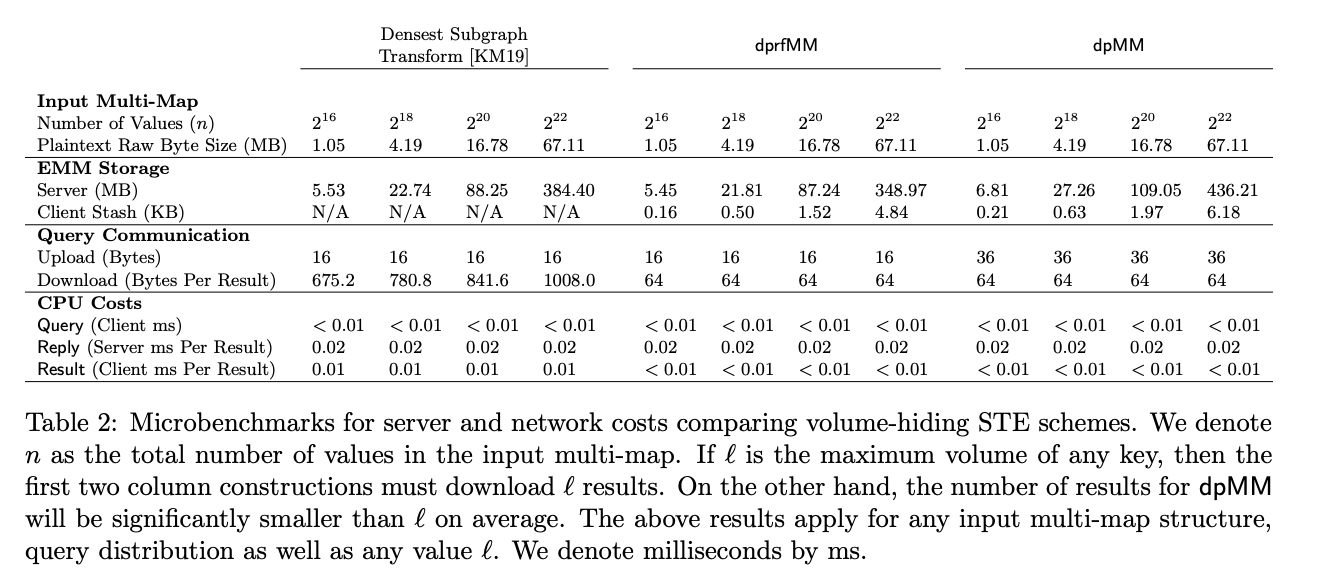
\includegraphics[width=4in]{imgs/exp.png}
\end{center}
\end{frame}

\setbeamercolor{background canvas}{bg=olive}
\begin{frame}

\begin{center}
{\color{yellow}
\Huge
Thank You

}
\end{center}

\vskip 1cm

{\color{yellow} ePrint:} {\tt https://eprint.iacr.org/2019/1292}

\vskip .3cm

{\color{yellow} CCS '19:} {\tt https://doi.org/10.1145/3319535.3354213}

\end{frame}

\end{document}


